% XCircuit output "linear_quantizer.tex" for LaTeX input from linear_quantizer.ps
\def\putbox#1#2#3{\makebox[0in][l]{\makebox[#1][l]{}\raisebox{\baselineskip}[0in][0in]{\raisebox{#2}[0in][0in]{#3}}}}
\def\rightbox#1{\makebox[0in][r]{#1}}
\def\centbox#1{\makebox[0in]{#1}}
\def\topbox#1{\raisebox{-\baselineskip}[0in][0in]{#1}}
\def\midbox#1{\raisebox{-0.5\baselineskip}[0in][0in]{#1}}
\begin{flushleft}
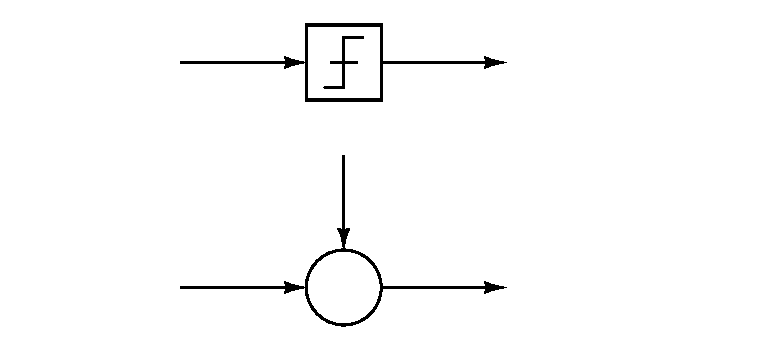
\epsfig{file=linear_quantizer.ps}\\
% translate x=296 y=160 scale 0.38
\putbox{0.60in}{1.85in}{\midbox{$x_a(n T_s)$}}%
\putbox{3.31in}{1.85in}{\midbox{$\mathcal{Q}\bigl[x_a(n T_s)\bigr]$}}%
\putbox{2.18in}{0.35in}{\centbox{\midbox{$\displaystyle\sum$}}}%
\putbox{0.60in}{0.35in}{\midbox{$x_a(nT_s)$}}%
\putbox{2.06in}{1.31in}{\midbox{$e(n)$}}%
\putbox{3.31in}{0.35in}{\midbox{$x_a(nT_s)+e(n)$}}%
\putbox{0.06in}{1.76in}{(a)}%
\putbox{0.06in}{0.26in}{(b)}%
\end{flushleft}
